% Chapter Template

\chapter{Projekt kwadrokoptera} % Main chapter title

\label{Chapter5} % Change X to a consecutive number; for referencing this chapter elsewhere, use \ref{ChapterX}

\lhead{Rozdział 5. \emph{Projekt kwadrokoptera}} % Change X to a consecutive number; this is for the header on each page - perhaps a shortened title

%----------------------------------------------------------------------------------------
%	SECTION 1
%----------------------------------------------------------------------------------------

\section{Wymagania techniczne}

Zaprojektowanie modelu kwadrokoptera nie należy do prostych zadań. Należy uwzględnić wiele czynników z zakresu mechaniki, elektroniki oraz informatyki mogących mieć wpływ na powodzenie projektu. Jako że autor pracy nie posiada żadnego doświadczenia związanego z konstrukcjami mechanicznymi oraz z budowaniem robotów, przy tworzeniu modelu kwadrokoptera największy nacisk położono na prostotę konstrukcji i zastosowanych rozwiązań. Docelowo starano się osiągnąć tanią uniwersalną konstrukcję, którą w przyszłości będzie można poszerzać o nowe moduły elektroniczne lub mechaniczne. Chcąc zdobyć jak największe doświadczenie w projektowaniu oraz programowaniu tego typu konstrukcji, w projekcie duży nacisk położono na własnoręczne zaprojektowanie układów elektronicznych oraz samodzielne opracowanie algorytmów sterujących.

Podstawowa lista wymagań technicznych wygląda następująco:

\begin{itemize}
	\item Niski koszt oraz uniwersalność konstrukcji.
	\item Ograniczona moc silników ze względów bezpieczeństwa.
	\item Czas lotu minimum 5 minut.
	\item Komunikacja radiowa o zasięgu minimum 5 metrów.
	\item Prosta, najlepiej gotowa konstrukcja mechaniczna.
	\item Prosta architektura elektroniki, oparta o mikrokontroler AVR.
	\item PCB zaprojektowane własnoręcznie.
	\item Algorytm napisany własnoręcznie.
\end{itemize}

\section{Koncepcja rozwiązania}

Zanim zaczęto analizować wymagania techniczne dotyczące samego kwadrokoptera, określono minimalną architekturę systemu, który musiał powstać, aby kwadrokopter mógł wznieść się w powietrze. Zdecydowano się na rozwiązanie, w skład którego wchodzą:

\begin{itemize}
	\item Kwadrokopter.
	\item Kontroler zdalnego sterowania.
	\item Aplikacja służąca do testów i strojenia parametrów lotu, przeznaczona na komputer PC.
\end{itemize}

\begin{figure}[H]
	\centering
	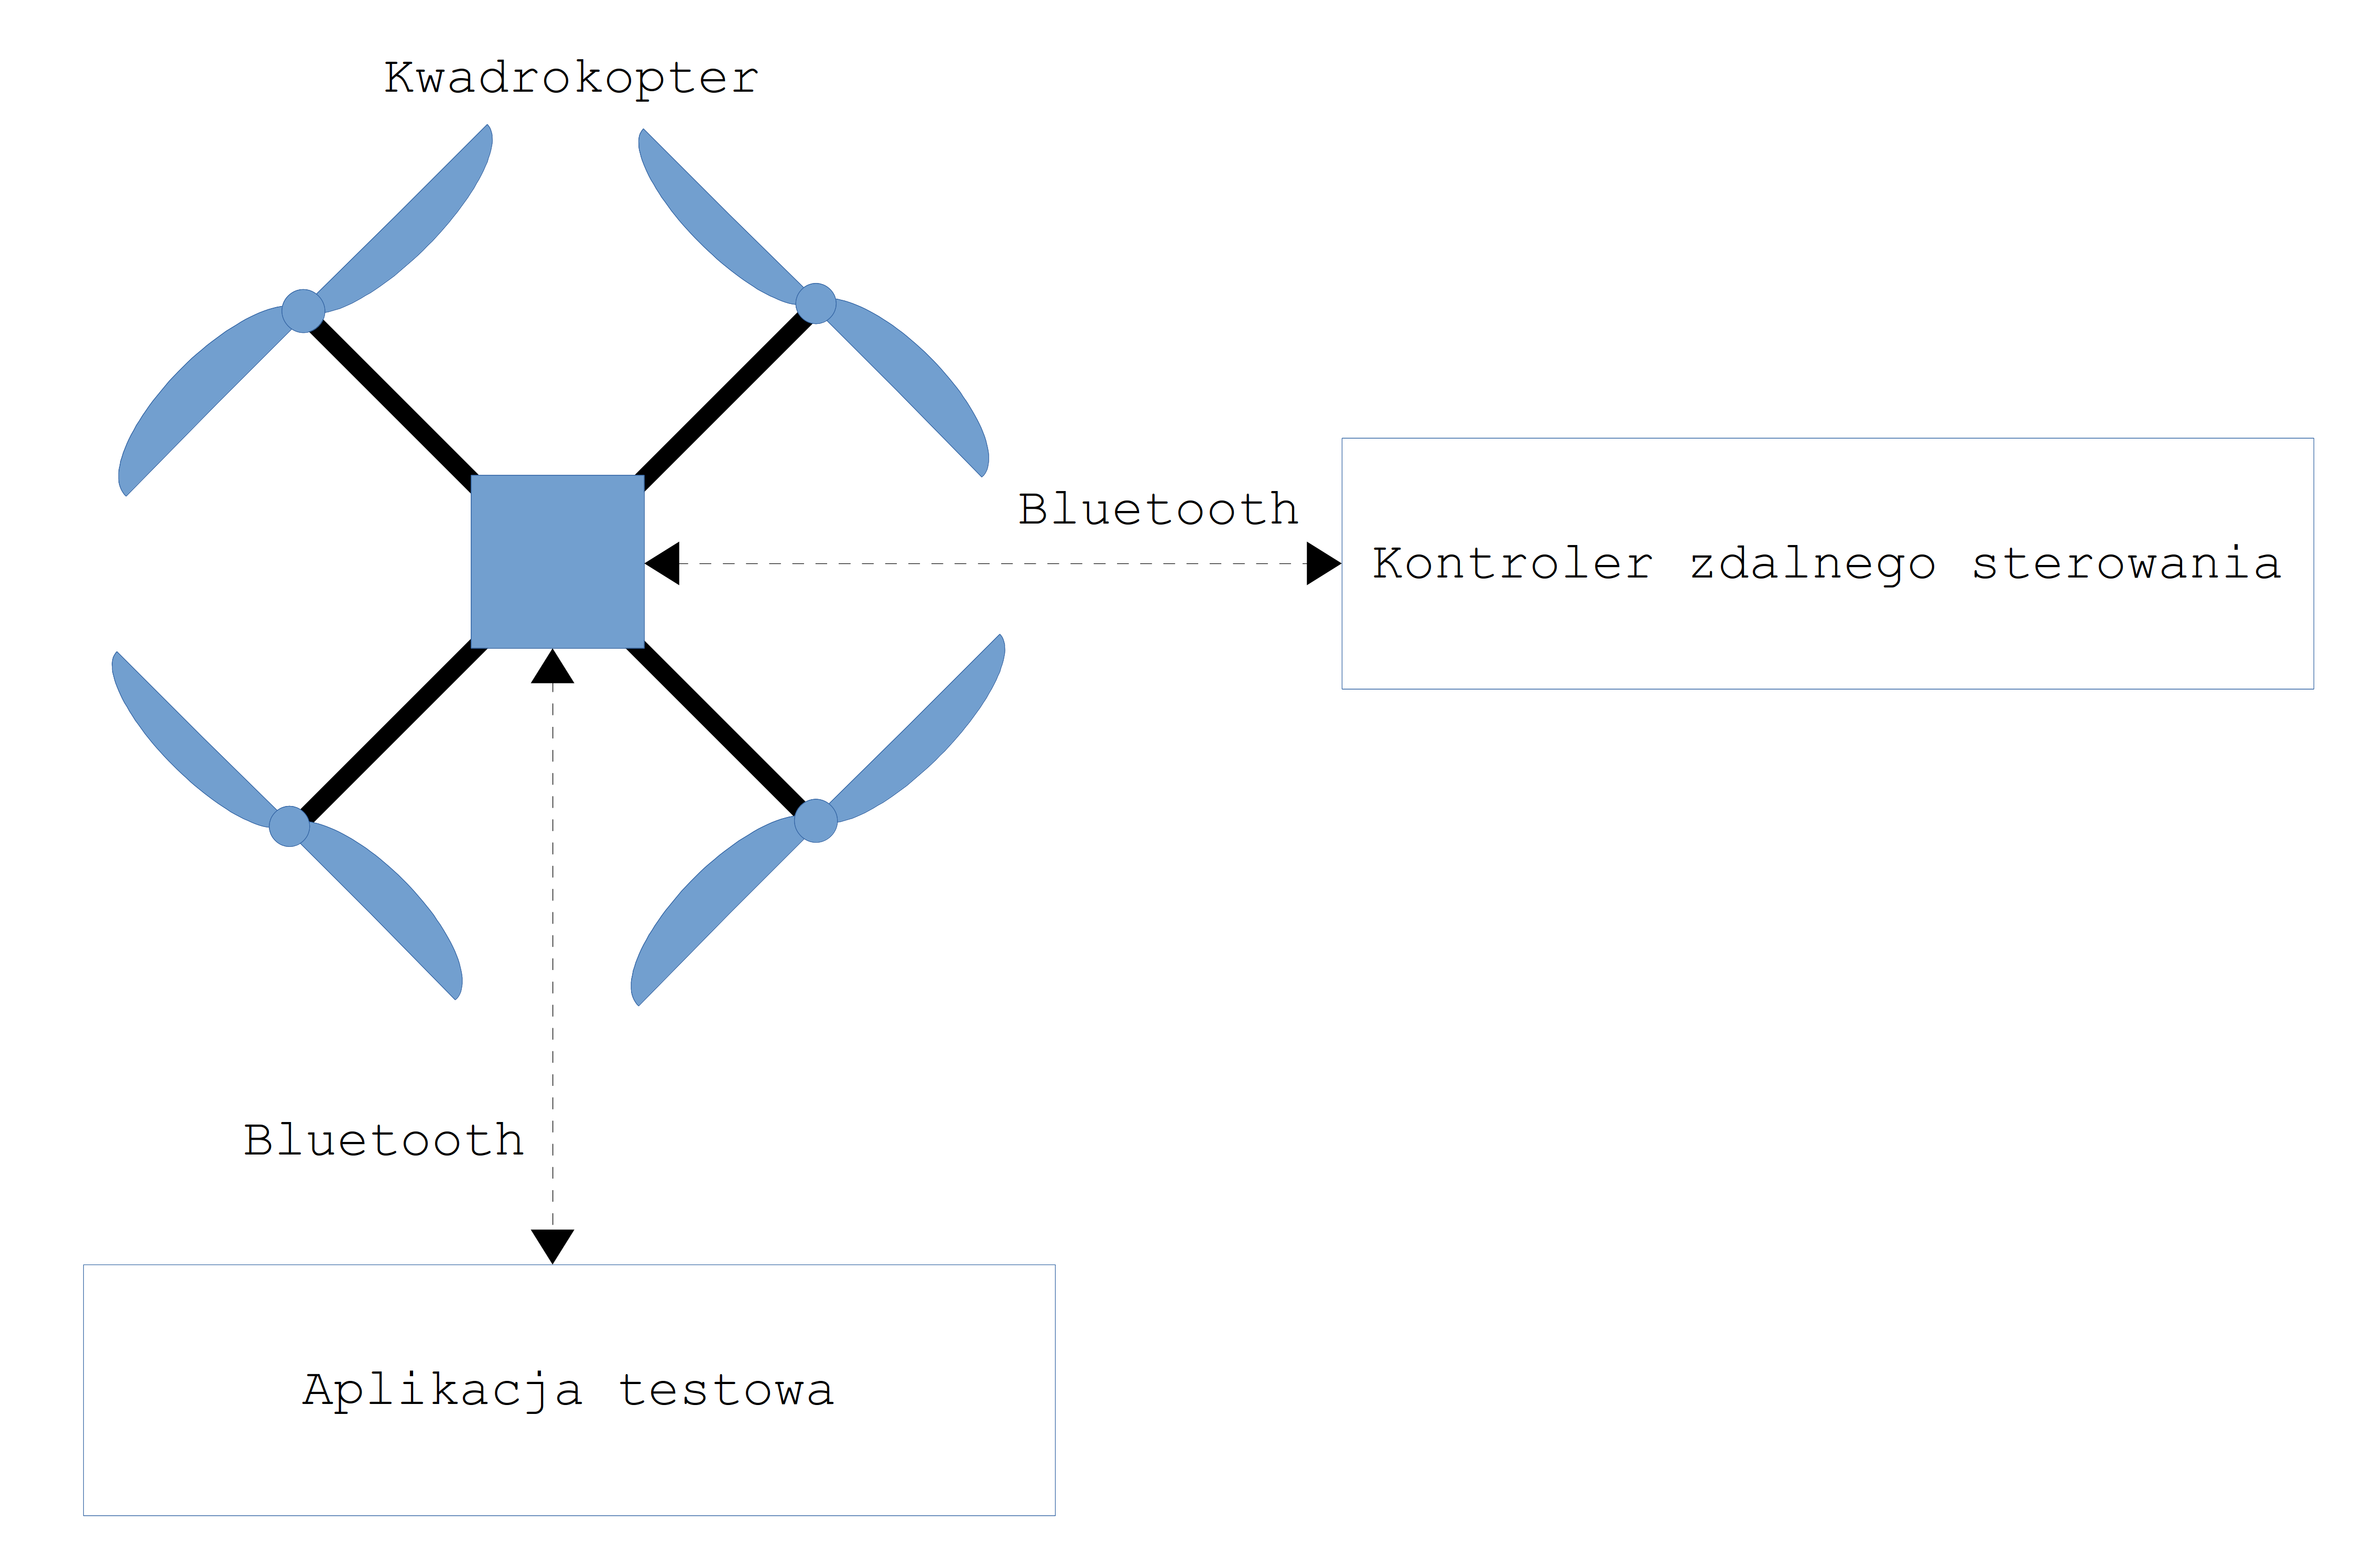
\includegraphics[scale=0.1]{Pictures/SchematSystemu.png}
		%\rule{35em}{0.5pt}
	\caption[Schemat blokowy systemu]{Schemat funkcjonalny projektowanego systemu}
	\label{fig:SchematSystemu}
\end{figure}



Rysunek ~\ref{fig:SchematSystemu} przedstawia ogólną architekturę zaprojektowanego systemu.

Kontroler zdalnego sterowania jest niezbędnym elementem systemu, za pomocą ktorego użytkownik wysyła sygnały sterujące kwadrokopterem drogą radiową. W obecnych czasach kontrolery lotu mogą stanowić bardzo skomplikowane systemy, wysyłające sygnały radiowe z użyciem wielu kanałów radiowych, co z reguły znajduje odzwierciedlenie w kosztach takiego urządzenia. W związku z tym, chcąc minimalizować koszty, przy projektowaniu systemu obrano inne podejście. Zdecydowano się na wykorzystanie telefonu komórkowego z systemem Android, wyposażonego w ekran dotykowy oraz wbudowany moduł Bluetooth. Dzięki napisaniu aplikacji w języku Java, która działa na wspomnianej platformie sprzętowej, można osiągnąć praktycznie zerowy (jako że autor projektu posiadał telefon przed projektowaniem systemu) koszt tworzenia kontrolera zdalnego sterowania. 

Podejście to ma wyraźne zalety w porównaniu do kupionego lub własnoręcznie opracowanego sprzętowego kontrolera zdalnego sterowania:

\begin{itemize}
	\item \textbf{W porównaniu do kupionego kontrolera lotu uzyskuje się:}
		\begin{itemize}
			\item brak konieczności dopasowywania tworzonego systemu do gotowego standardu radiowej transmisji sygnałów sterujących,
			\item dużo niższy koszt kontrolera.
		\end{itemize}
	\item \textbf{W porównaniu do własnoręcznie wykonanego sprzętowego kontrolera lotu uzyskuje się:}
		\begin{itemize}
			\item krótszy czas tworzenia kolejnych prototypów,
			\item niższy koszt kontrolera.
		\end{itemize}
\end{itemize}

Zanim nastąpi moment uniesienia się kwadrokoptera w powietrze, należy najpierw nastroić regulatory zaimplementowane w algorytmie kontroli lotu. Podczas projektowania systemu zdecydowano się powierzyć tę rolę oddzielnej aplikacji przeznaczonej na komputer PC. Stało się tak między innymi za sprawą dużej liczby danych, które taka aplikacja potencjalnie musi wysyłać oraz przetwarzać. Chcąc mieć możliwość ustawiania licznych parametrów algorytmu, uzytkownik powinien mieć możliwośc ujrzenia tych parametrów jednocześnie, co dyskfalifikuje ekran telefonu do wykorzystania w takiej roli. Ponieważ w przypadku projektowania kontrolera zdalnego sterowania zdecydowano się na wykorzystanie interfejsu Bluetooth, mając na uwadze prostotę i niski koszt całego systemu, aplikacja testowa przeznaczona na komputer również wykorzystuje ten interfejs.

Kwadrokopter ma możliwość komunikacji z jednym z pozostałych elementów systemu w danym czasie, a zatem użytkownik może albo dokonywać kalibracji algorytmu kontroli lotu, albo wysyłania sygnałów sterujących lotem kwadrokoptera.

Po zaproponowaniu ogólnej architektury systemu, można przejść do projektowania systemu sterującego kwadrokoptera. Schemat blokowy systemu przedstawia rysunek~\ref{fig:QuadroSchematIdeowy}.

\begin{figure}[H]
	\centering
	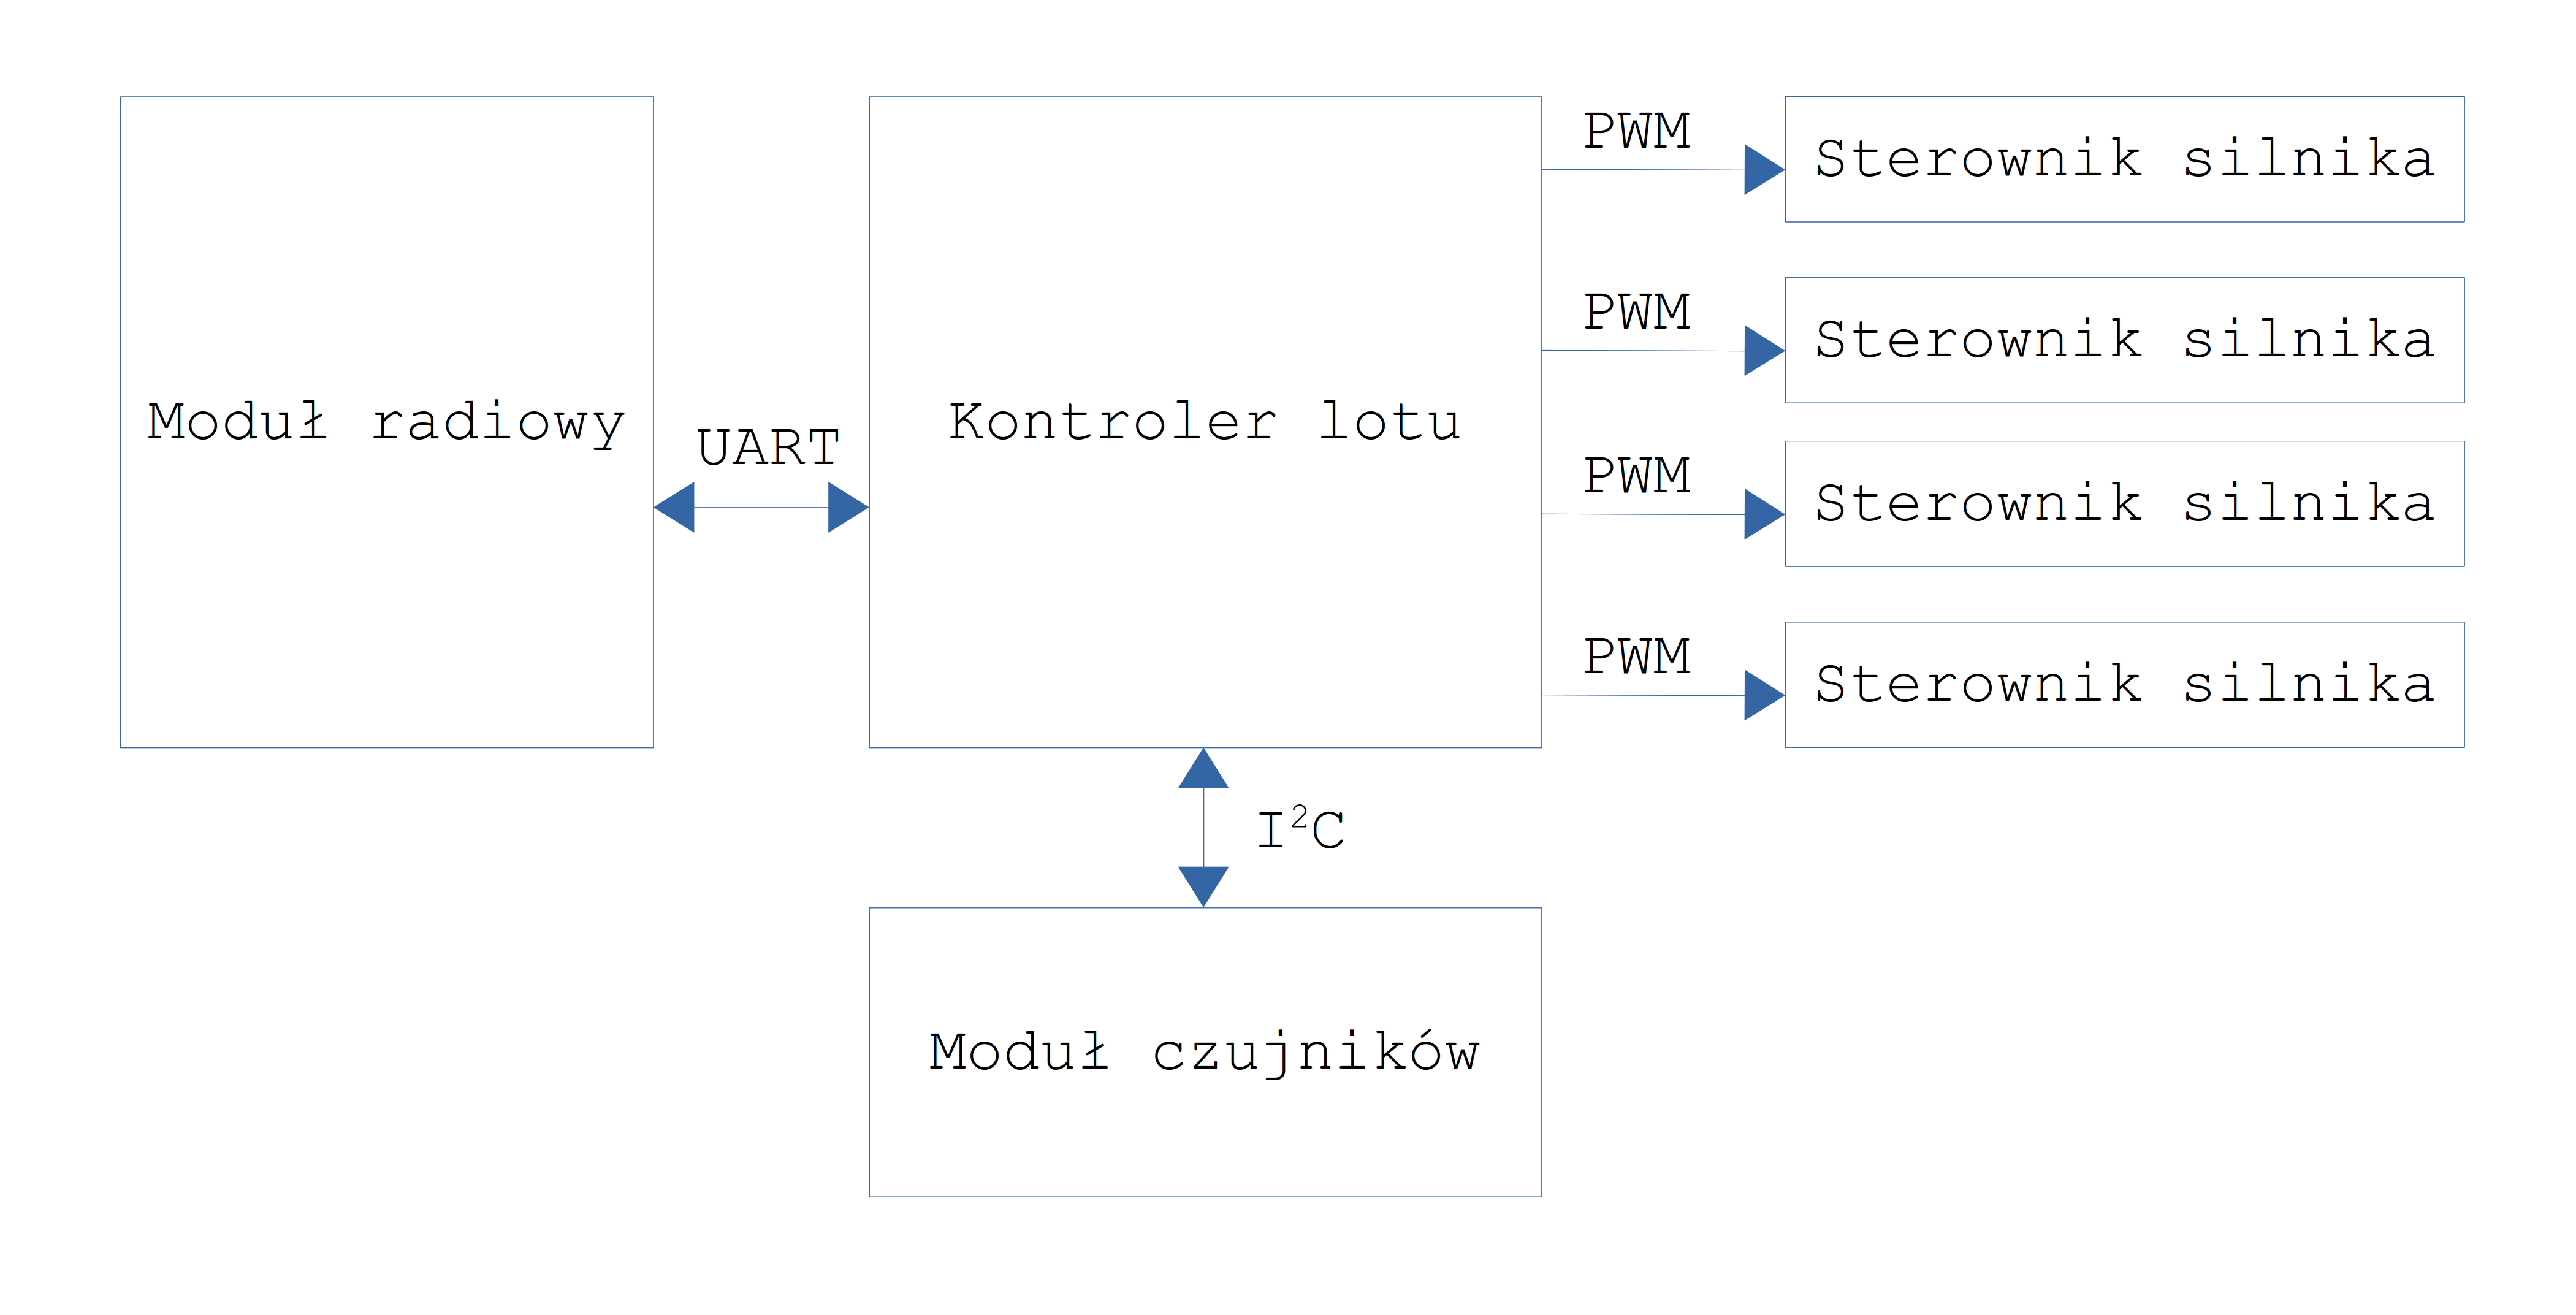
\includegraphics[scale=0.1]{Pictures/QuadroSchematIdeowy.png}
		%\rule{35em}{0.5pt}
	\caption[Schemat blokowy kwadrokoptera]{Schemat blokowy systemu sterującego kwadrokoptera}
	\label{fig:QuadroSchematIdeowy}
\end{figure}

Przy projektowaniu ekeltroniki kwadrokoptera główną ideą, jaka przyświecała autorowi projektu, była uniwersalność konstrukcji, tak aby można ją było w przyszłości rozbudowywać. Dlatego też zdecydowano się na modułową konstrukcję, składającą się z czterech głównych elementów:
\begin{itemize}
	\item Kontroler lotu
	\item Moduł komunikacji radiowej
	\item Moduł czujników
	\item Kontrolery silników
\end{itemize}

\subsection{Kontroler lotu}
Kontroler lotu jest jednostką odpowiedzialną za utrzymanie kwadrokoptera w powietrzu. Jak widać na rysunku ~\ref{fig:QuadroSchematIdeowy}, komunikuje się on z modułem czujników za pomocą magistrali I\textsuperscript{2}C oraz z modułem komunikacji radiowej za pomocą interfejsu UART. Ponadto musi on generować sygnały do sterowników silników zgodne z modelarskim standardem PWM opisanym w~\ref{Chapter2} rozdziale. Wybór mikrokontrolera użytego w tym module padł na układ z rodziny AVR - ATmega328p. Poniżej przedstawiono podstawowe cechy użytego mikrokontrolera:

\begin{itemize}
	\item Maksymalna częstotliwość taktowania 20MHz.
	\item Sześć niezależnych kanałów PWM.
	\item Interfejs USART.
	\item Interfejs I\textsuperscript{2}C.
	\item Napięcie zasilania 1.8V - 5.5V.
	\item 32kB pamięci programu.
	\item 2kB pamięci RAM.
	\item Dostępność w obudowie TQFP-32.
\end{itemize}

Jak zatem widać, układ ten spełna wszystkie wymagania stawiane przed jednostką kontroli lotu, posiadając niezbędne interfejsy komunikacyjne, odpowiednią liczbę kanałów PWM, zdolnych do generowania sygnałów dla sterowników silników oraz pojemność pamięci programu i danych pozwalającą na implementację stosunkowo złożonych algorytmów. Niskie minimalne napięcie zasilania pozwala na zasilanie tego mikrokontrolera bezpośrednio z akumulatora litowo-polimerowego, dzięki czemu można uniknąć stosowania przetwornic podwyższających napięcie.

\subsection{Moduł komunikacji radiowej}
Moduł komunikacji radiowej jest odpowiedzialny za odbieranie sygnałów sterujących wysyłanych przez użytkownika urządzenia. W projekcie zdecydowano się na transmisję danych sterujących i danych używanych do strojenia algorytmu kwadrokoptera za pomocą jednego modułu, najprościej jest więc przesyłać dane w postaci cyfrowej zgodnie z protokołem opracowanym specjalnie do tego zadania. Wybór padł na moduł HC-05 ze względu na następujące parametry:

\begin{itemize}
	\item Napięcie zasilania 3.3V.
	\item Prąd pobierany podczas transmisji 8mA.
	\item Maksymalny zasięg 10m.
	\item Komunikacja poprzez interfejs UART.
	\item Niska cena.
\end{itemize}

\begin{figure}[H]
	\centering
	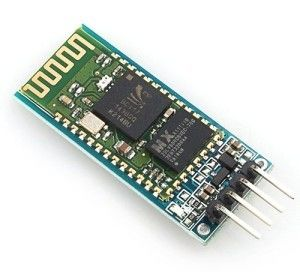
\includegraphics[scale=0.7]{Pictures/HC-05.jpg}
		%\rule{35em}{0.5pt}
		\caption[Moduł Bluetooth HC-05]{Moduł Bluetooth HC-05}
	\label{fig:hc-05}
\end{figure}

Dzięki tym cechom możliwe jest zasilanie modułu bezpośrednio z akumulatora litowo-polimerowego zamontowanego w kwadrokopterze oraz przeysłanie danych sterujących i kalibracyjnych za pomocą prostego protokołu.

\subsection{Moduł czujników}
Moduł czujników odpowiedzialny jest za dostarczanie informacji o rzeczywistych parametrach fizycznych (położenie kątowe, prędkość kątowa) kwadrokoptera. Obecnie na rynku można spotkać rozmaite moduły czujników przeznaczone do konstrukcji latających, oferujące akcelerometry, żyroskopy, magnetometry i barometry. Wiele z tych konstrukcji ma jednak stosunkowo wysoką cenę, a ich popularność wśród użytkowników jest niewielka. Wybór padł więc na bardzo popularny a co za tym idzie tani moduł oparty o układ scalony MPU-6050, oferujący następujące parametry:

\begin{itemize}
	\item 3-osiowy Akcelerometr i 3-osiowy żyroskop zintegrowane w jednej obudowie.
	\item Uniwersalny interfejs komunikacyjny I\textsuperscript{2}C.
	\item Napięcie zasilania 2.4V - 3.5V.
	\item Prąd pobierany w trakcie pracy poniżej 5.5mA.
	\item Szeroki zakres konfiguracji skali pomiarowej czujników.
		\begin{itemize}
			\item Akcelerometr $\pm 2g$, $\pm 4g$, $\pm 8g$, $\pm 16g$
			\item Żyroskop $\pm 250^{\circ}/s$, $\pm 500^{\circ}/s$, $\pm 1000^{\circ}/s$, $\pm 2000^{\circ}/s$
		\end{itemize}
	\item Niewielkie wymiary fizyczne modułu.
\end{itemize}

\begin{figure}[H]
	\centering
	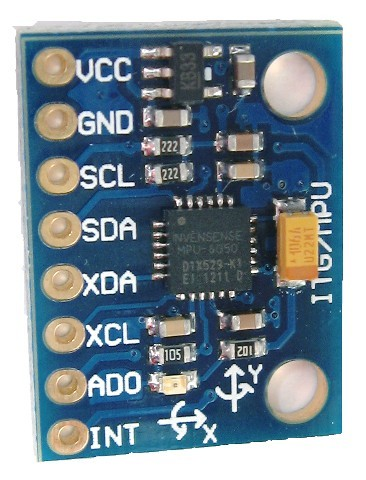
\includegraphics[scale=0.6]{Pictures/mpu-6050.jpg}
		%\rule{35em}{0.5pt}
		\caption[Moduł czujników MPU-6050]{Moduł czujników MPU-6050}
	\label{fig:mpu-6050}
\end{figure}

\subsection{Kontrolery silników}
Kontrolery silników odpowiedzialne są za odbieranie sygnałów sterujących wysyłanych przez kontroler lotu i przetwarzanie ich na sygnał PWM, sterujący silnikiem. Przy opracowaniu koncepcji omawianych modułów, największy nacisk położono na prostotę i niewielkie wymiary konstrukcji. Procesor użyty w kontrolerze powinien posiadać minimalnie jedno wejście cyfrowe podłączone do kontrolera lotu, oraz jedno wyjście cyfrowe generujące sygnał PWM sterujący silnikiem. Wybór padł na mikrokontroler ATtiny85 ze względu na następujące cechy:

\begin{itemize}
	\item Dwa niezależne kanały PWM.
	\item Zewnętrzne źródła przerwania.
	\item Napięcie pracy 1.8V - 5.5V.
	\item Dostępność w obudowie SOIC-8.
\end{itemize}

Wybrany mikrokontroler spełnia wszystkie stawiane przed nim wymagania, oferując przy okazji ilość obszar znacznie przekraczający wymagania najprostszego algorytmu sterującego silnikami, co umożliwi potencjalny rozwój oprogramowania w przyszłości.

\section{Opis układowy}

\subsection{Kontroler lotu}

\begin{figure}[H]
	\centering
	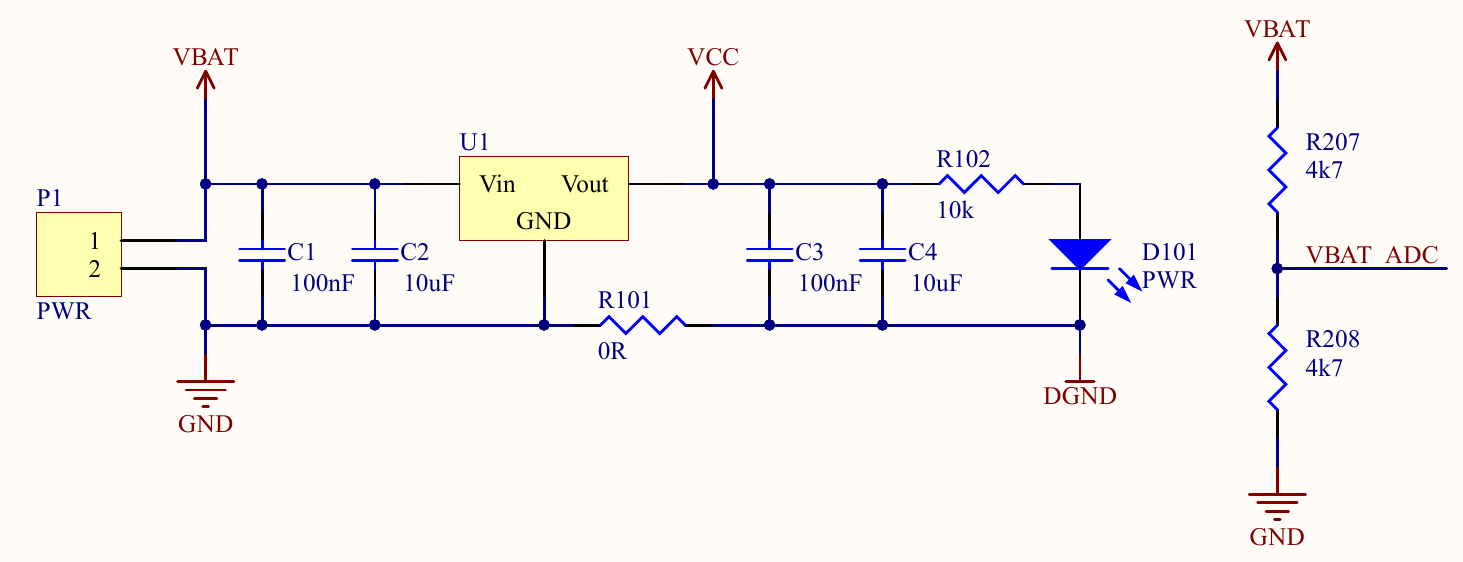
\includegraphics[scale=0.4]{Pictures/QuadroController_PWR_C.png}
		%\rule{35em}{0.5pt}
		\caption[Kontroler lotu - blok zasilania]{Kontroler lotu - blok zasilania}
	\label{fig:QuadroControllerPWR}
\end{figure}

Rysunek ~\ref{fig:QuadroControllerPWR} przedstawia blok zasilania kontrolera lotu kwadrokoptera. Składa się on ze stabilizatora LDO, o minimalnym napięciu wejściowym w okolicach 3.5V, dającego na wyjściu 3.3V. Tak niskie napięcie wejściowe niezbędne było w celu zasilania kontrolera bezpośrednio z akumulatora litowo-polimerowego. Poza stabilizatorem napięcia, blok zasilania składa się kondensatorów filtrujących napięcie, diody wskazującej obecność napięcia zasilania oraz dzielnika rezystancyjnego, wykorzystywanego przez mikrokontroler do pomiaru napięcia głównego akumulatora. Jako że ujemny biegun akumulatora będzie bezpośrednio podłączony do silników kwadrokoptera, mogą na nim występować różne zakłócenia związane z ich pracą. Dlatego też w obrębie płytki kontrolera lotu utworzono masę cyfrową, połączoną z masą analogową (ujemnym biegunem akumulatora) za pomocą rezystora R101.

\begin{figure}[H]
	\centering
	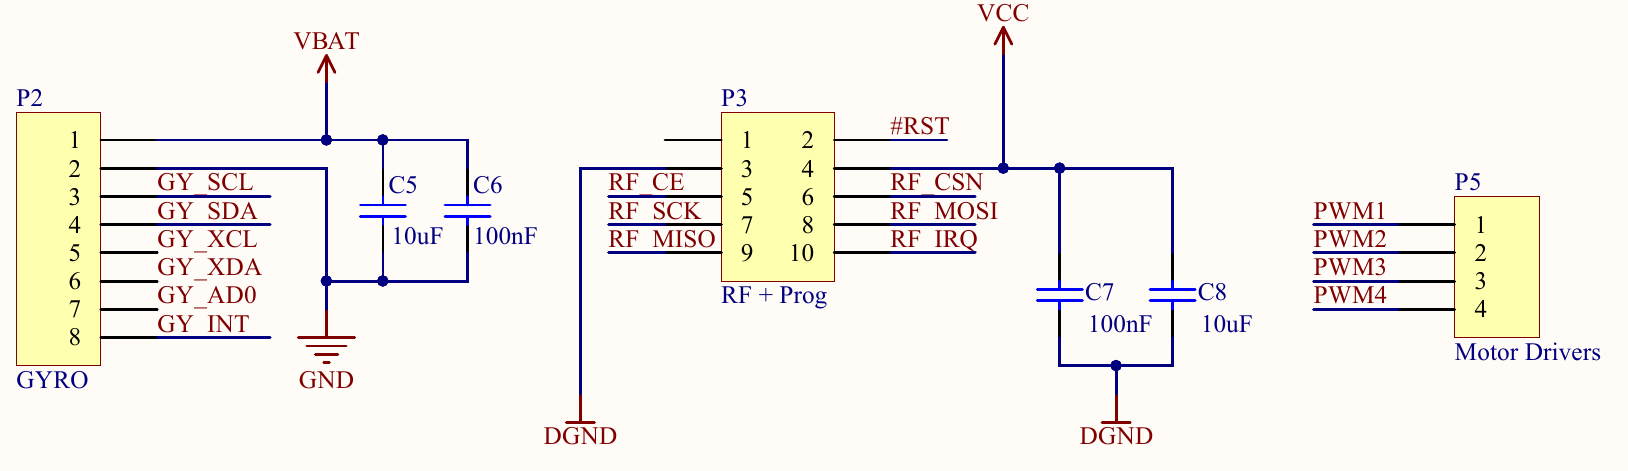
\includegraphics[scale=0.36]{Pictures/QuadroController_Connector_C.png}
		%\rule{35em}{0.5pt}
		\caption[Kontroler lotu - złącza sygnałowe]{Kontroler lotu - złącza sygnałowe}
	\label{fig:QuadrotorControllerConnectors}
\end{figure}

Rysunek ~\ref{fig:QuadrotorControllerConnectors} przedstawia złącza zamontowane na płytce kontrolera lotu. 
\begin{itemize}
	\item Złącze P2 przeznaczone jest dla modułu czujników MPU-6050. Ponieważ moduł ten posiada własny stabilizator napięcia zasilania do złącza doprowadzone jest bezpośrednio zasilanie z akumulatora wraz z niezbędnymi kondensatorami filtrującymi zasilanie. Z pozostałych wyprowadzeń modułu czujników, używane są jedynie linie interfejsu I\textsuperscript{2}C oraz wyjście sygnału przerwania (GY\_INT).
	\item Złącze P3 przeznaczone jest do programowania mikrokontrolera wykorzystanego w kontrolerze lotu oraz zostało przewidziane jako potencjalne złącze modułu radiowego, działającego w paśmie 2.4GHz i komunikującego się z mikrokontrolerem za pomocą interfejsu SPI.  
	\item Złącze P5 służy do wyprowadzenia sygnałów PWM sterujących silnikami, skąd następnie trafiają do kontrolerów silników.
\end{itemize}

\begin{figure}[H]
	\centering
	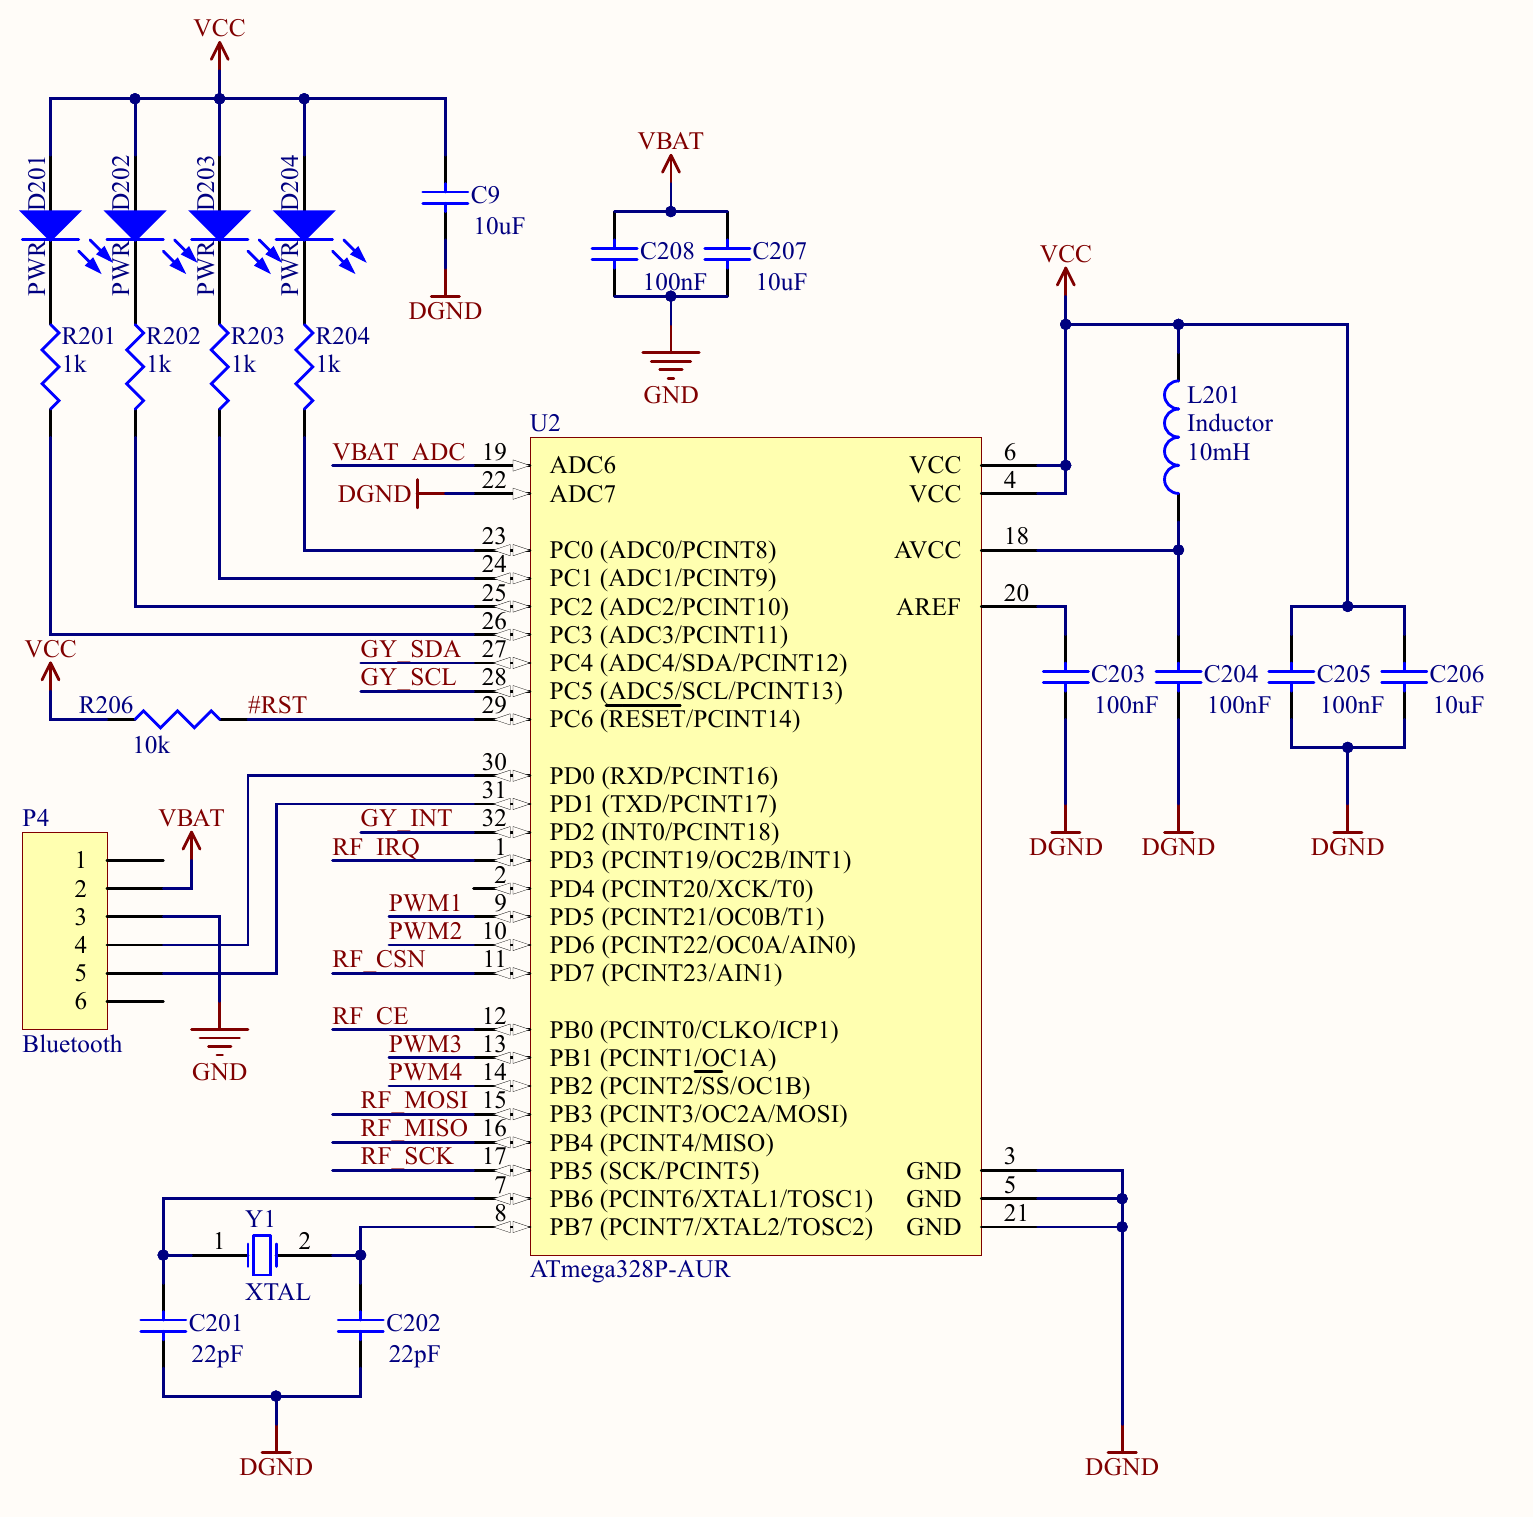
\includegraphics[scale=0.37]{Pictures/QuadroController_Main_C.png}
		%\rule{35em}{0.5pt}
		\caption[Kontroler lotu - jednostka centralna]{Kontroler lotu - jednostka centralna}
	\label{fig:QuadrotorControllerMain}
\end{figure}

Rysunek ~\ref{fig:QuadrotorControllerMain} przedstawia główny schemat ideowy kontrolera lotu. Składa się on z mikrokontrolera ATmega328P taktowanego zewnętrznym rezonatorem kwarcowym o częstotliwości 16MHz. Do złącza P4 podłączono wyprowadzenia interfejsu UART, za pomocą którego realizowana jest komunikacja z modułem Bluetooth. Pozostałe wyprowadzenia procesora wykorzystane są jako interfejsy komunikacyjne (I\textsuperscript{2}C, SPI) a także jako wyjścia sygnałów trafiających do sterowników silników (PWM1 - PWM4). Piny PC0 - PC4 zostały użyte do sterowania diodami LED, służącymi jako wskaźnik działania programu. Wejście ADC6 zostało wykorzystane do pomiaru napięcia akumulatora litowo-polimerowego, tak aby kontroler lotu mógł wysłać do pilota ostrzeżenie o konieczności ładowania. 

\begin{figure}[H]
	\centering
	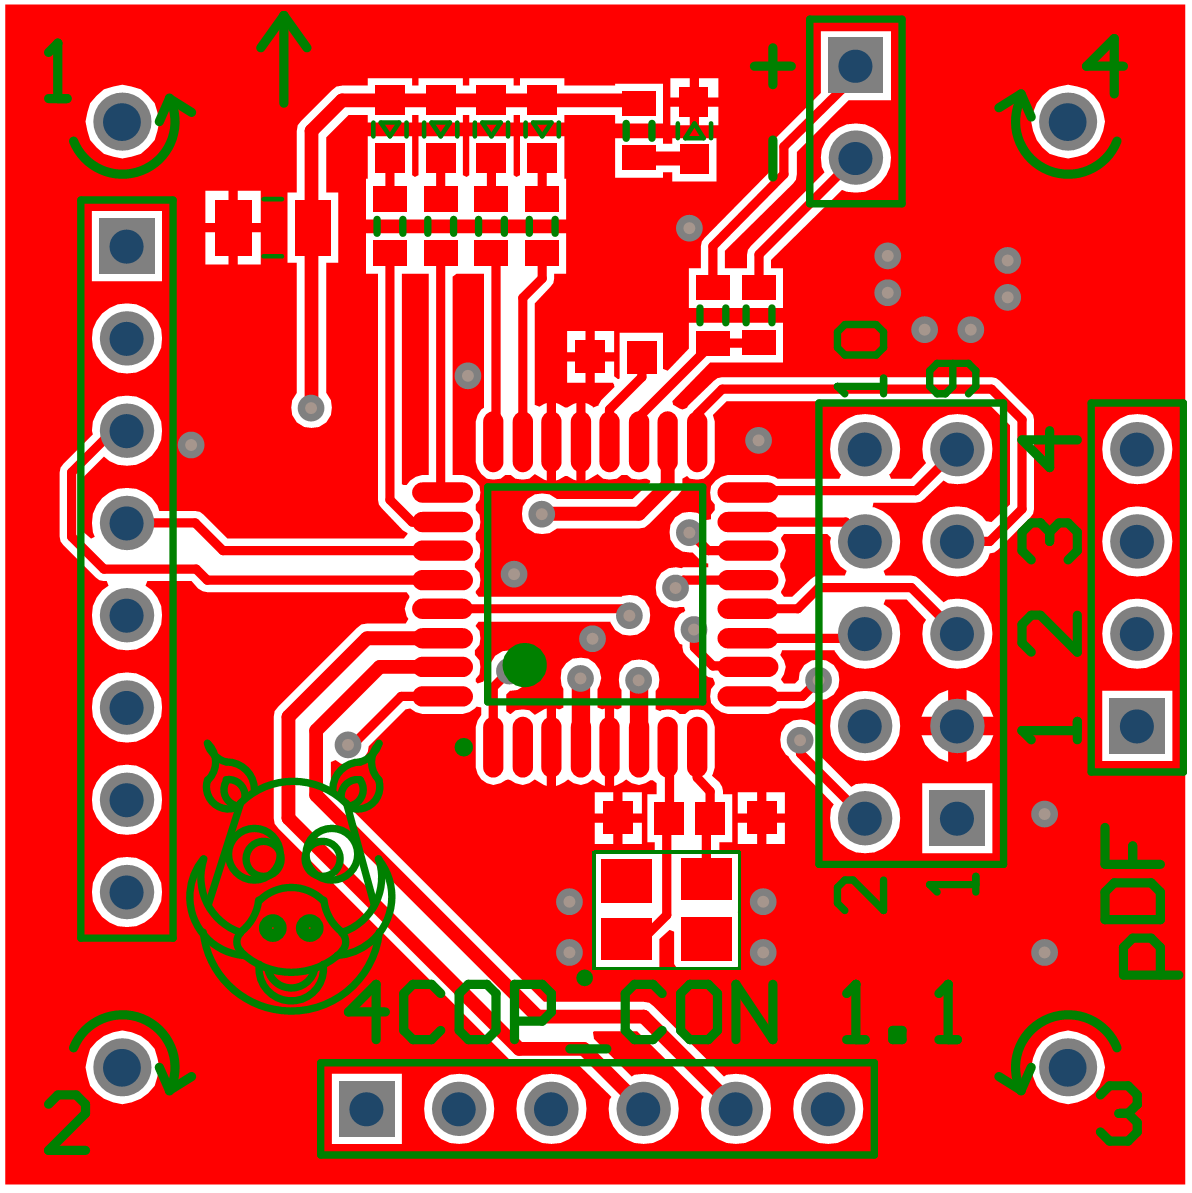
\includegraphics[scale=0.24]{Pictures/QuadrotorControllerPCB_TOP.png}
		%\rule{35em}{0.5pt}
		\caption[Kontroler lotu - płytka PCB, warstrwa górna]{Kontroler lotu - płytka PCB, warstwa górna}
	\label{fig:QuadrotorControllerPCB_TOP}
\end{figure}

\begin{figure}[H]
	\centering
	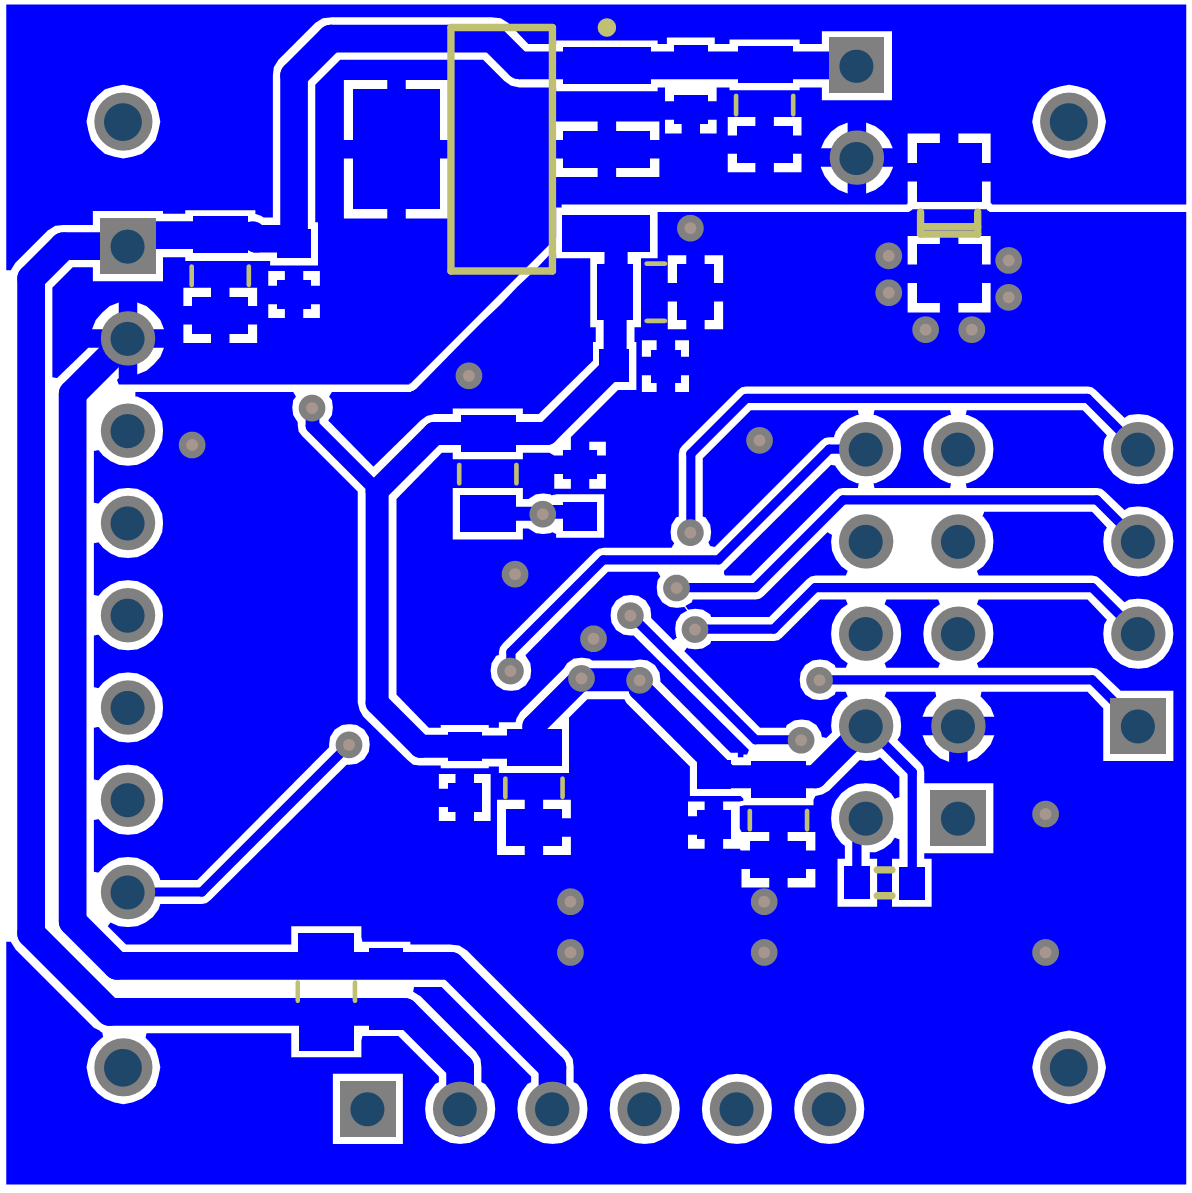
\includegraphics[scale=0.24]{Pictures/QuadrotorControllerPCB_Bottom.png}
		%\rule{35em}{0.5pt}
		\caption[Kontroler lotu - płytka PCB, warstrwa dolna]{Kontroler lotu - płytka PCB, warstwa dolna}
	\label{fig:QuadrotorControllerPCB_Bottom}
\end{figure}

Rysunki ~\ref{fig:QuadrotorControllerPCB_TOP} oraz ~\ref{fig:QuadrotorControllerPCB_Bottom} przedstawiają górną i dolną wartstwę płytki PCB kontrolera lotu. Na warstwie górnej zamontowany jest mokrokontroler wraz ze wszystkimi złączami, które są wykorzystywane przez zewnętrzne moduły. Jedynymi liniami, przy prowadzeniu których trzeba było zwrócić uwagę na ograniczenie długości, są linie od rezonatora kwarcowego, dlatego też został on umieszczony na tej samej warstwie co mikrokontroler, tuż pod nim, tak aby linie sygnału zegarowego miały minimalną długość oraz aby nie było konieczności prowadzenia ich przez przelotki. Pozostałe sygnały ze względu na niewielką maksymalną częstotliwość nie musiały spełniać reguł odnośnie wyrównania długości ścieżek lub dopasowania impedancji. Warstwa dolna płytki drukowanej została przeznaczona w głównej mierze na montaż elementów z bloku zasilania (stabilizator LDO, kondensatory filtrujące napięcie) oraz poprowadzenie linii zasilania. Na tej warstwie widac również podział masy zasilania na masę analogową oraz cyfrową połączone rezystorem R101. Masa analogowa została rozprowadzona w ten sposób, aby nie przechodziła pod żadnymi ważnymi liniami sygnałowymi (I\textsuperscript{2}C, SPI) oraz co ważniejsze pod liniami sygnału zegarowego pochodzącego od rezonatora kwarcowego. Rozmiar płytki drukowanej oraz rozmieszczenie otworów montażowych zostały dobrane tak, aby ułatwić montaż kontrolera lotu na ramie kwadrokoptera wybranej do tego projektu.

\subsection{Sterownik silnika}

\begin{figure}[H]
	\centering
	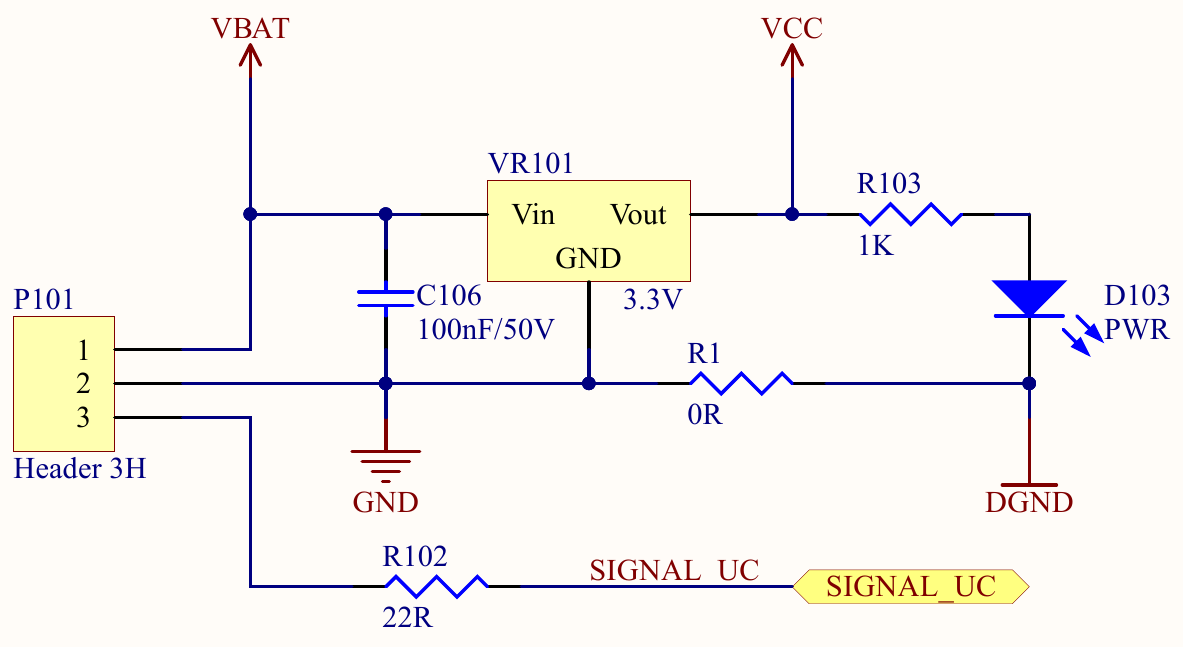
\includegraphics[scale=0.45]{Pictures/MotorController_PWR_C.png}
		%\rule{35em}{0.5pt}
		\caption[Sterownik silnika - blok zasilania]{Sterownik silnika - blok zasilania}
	\label{fig:MotorDriver_PWR}
\end{figure}

Rysunek ~\ref{fig:MotorDriver_PWR} przedstawia blok zasilania sterownika silnika. Jest on bardzo podobny do zasilania kontrolera lotu i składa się ze stablilizatora LDO o minimalnym napięciu wejściowym 3.5V, rezystora R1 łączącego masę analogową i cyfrową układu, diody informującej o obecności napięcia zasilania oraz diody sygnalizacyjnej, używanej jako wskaźnik działania programu wgranego do mikrokontrolera. Złącze P101 służy do podłączenia napięcia zasilania (piny 1 oraz 2) oraz do podłączenia sygnału PWM informującego moduł o zadanej prędkości obrotowej silnika.

\begin{figure}[H]
	\centering
	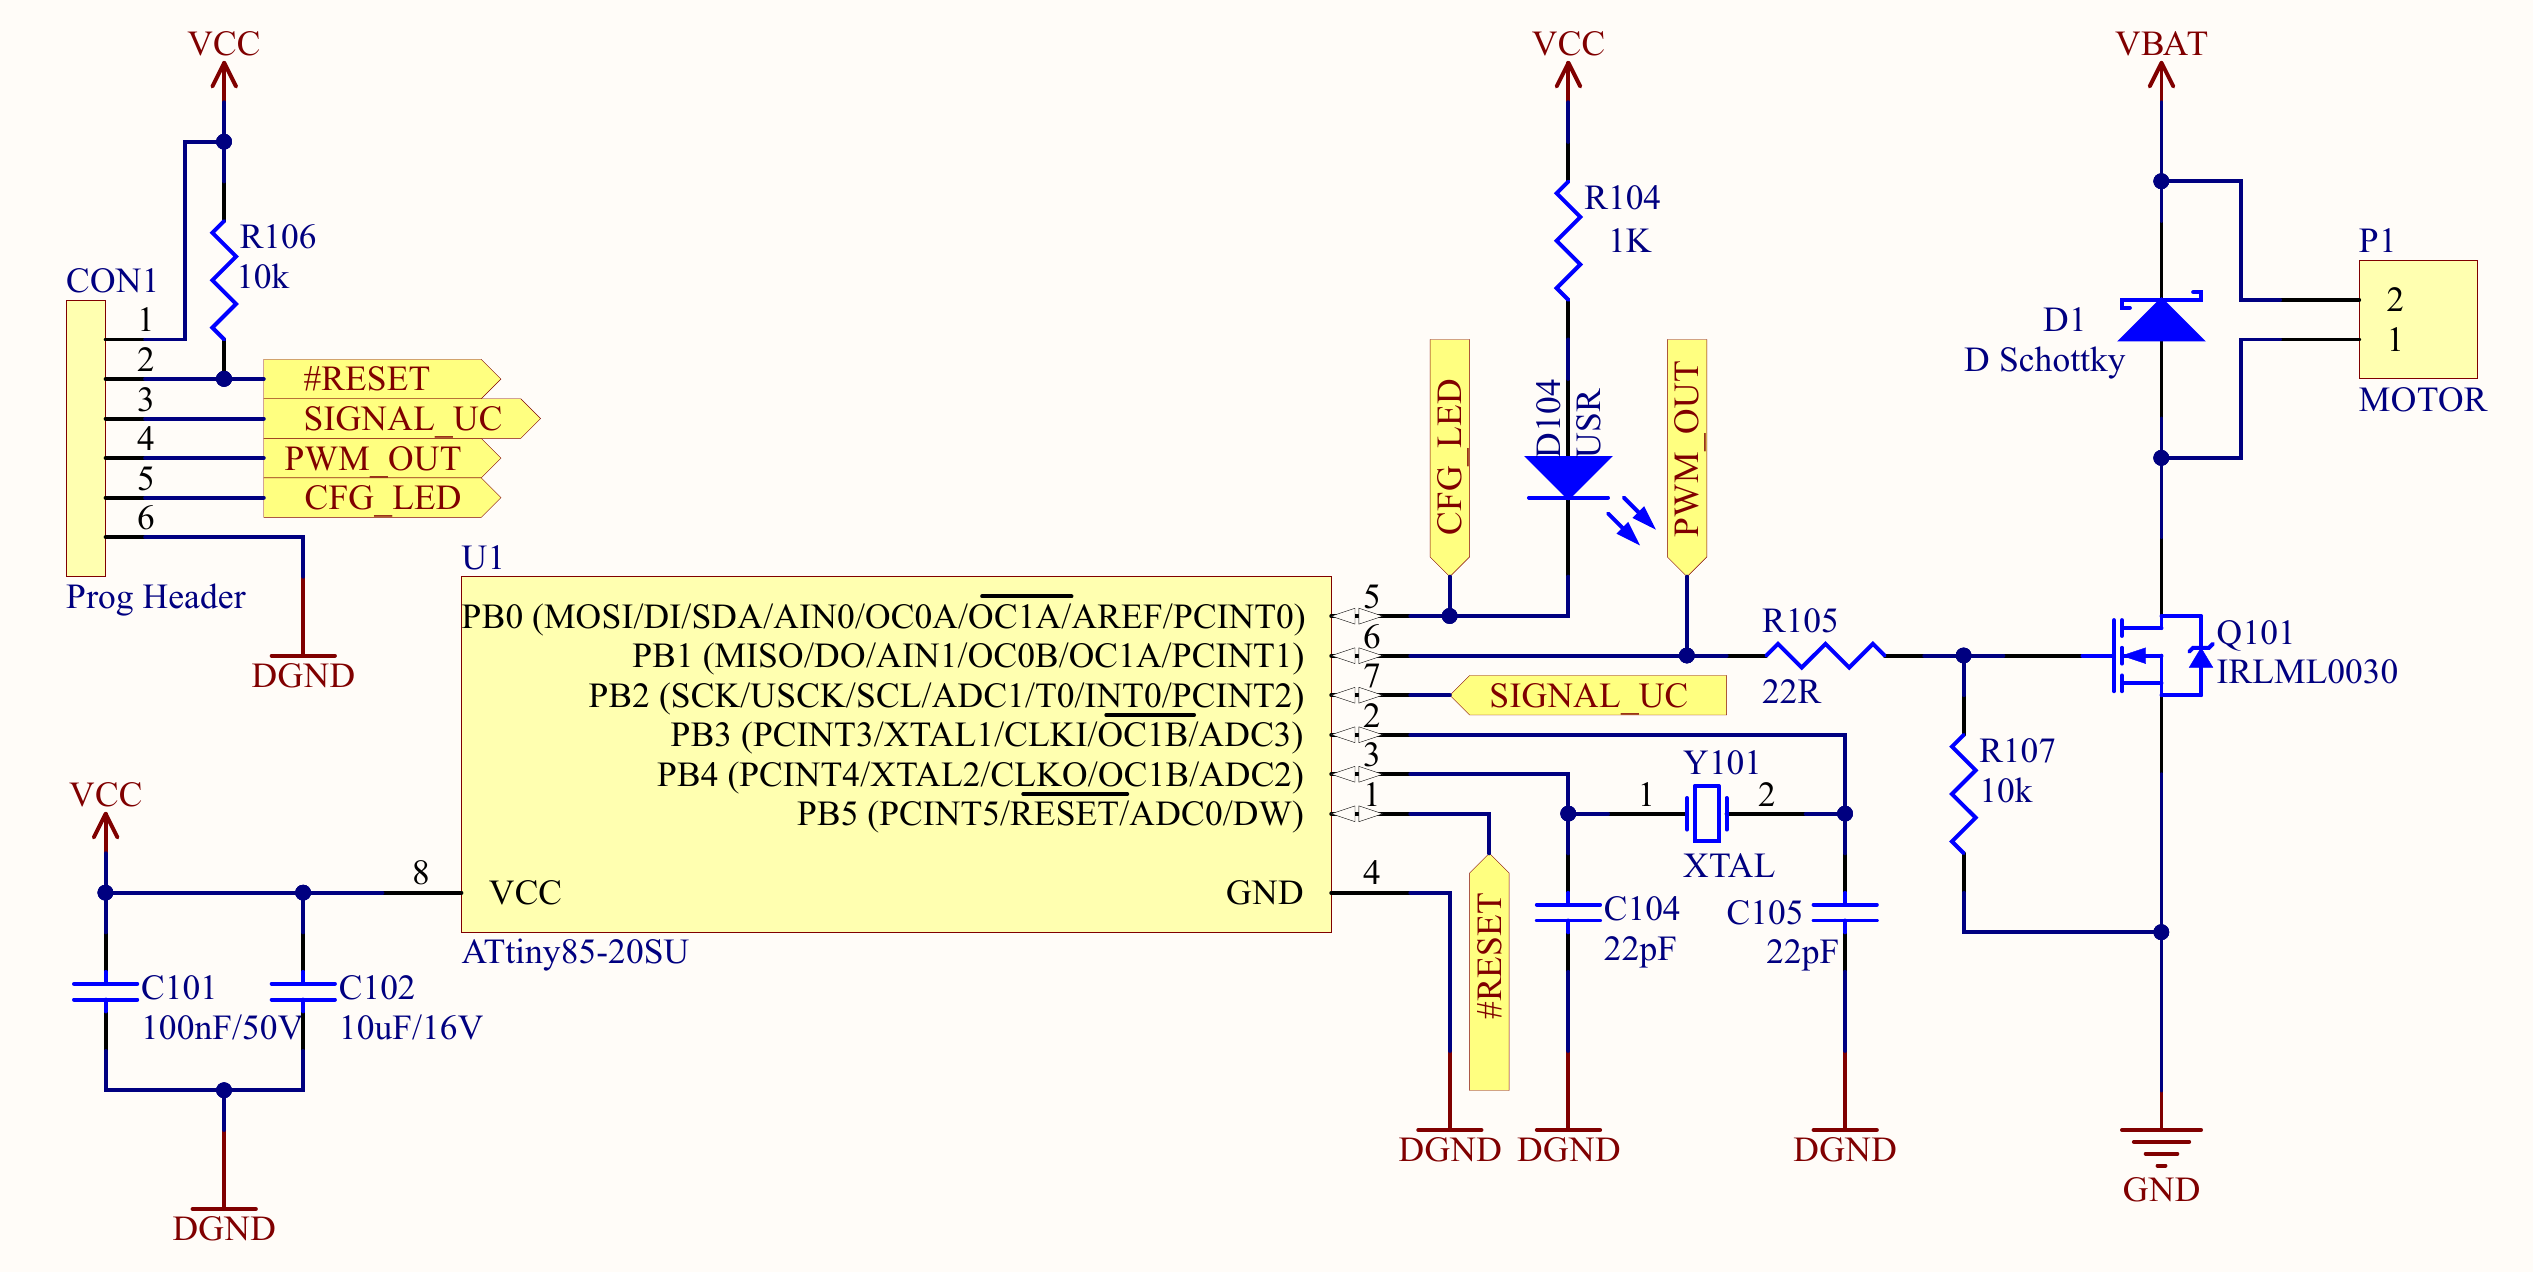
\includegraphics[scale=0.30, angle=90]{Pictures/MotorController_Main_C.png}
		%\rule{35em}{0.5pt}
		\caption[Sterownik silnika - jednostka centralna]{Sterownik silnika - jednostka centralna}
	\label{fig:MotorDriver_MAIN}
\end{figure}

Rysunek ~\ref{fig:MotorDriver_MAIN} przedastawia główny schemat kontrolera silnika. Składa się on z mikrokontrolera ATtiny85 taktowanego zewnętrznym rezonatorem o częstotliwości 12MHz. Sygnał PWM pochodzący z kontrolera lotu przechodzi przez rezystor R102 tworzący z pojemnością wejścia mikrokontrolera filtr dolnoprzepustowy tłumiący część zakłóceń. Następnie trafia on na pin mikrokontrolera zdolny do generowania zewnętrznego przerwania. Z mikrokontrolera wyprowadzony jest sygnał PWM  trafiający na tranzystor Q101 sterujący silnikiem. Rezystor R105 zapobiega impulsom prądowym, które występują podczas ładowania i rozładowywania pasożytniczej pojemności bramki tranzystora, natomiast rezystor R107 wymusza niski stan na bramce tranzystora (co za tym idzie wyłączenie silnika) przy braku sygnału sterującego ze strony mikrokontroelra. Dioda Schottky'ego D1 ma za zadanie niwelowanie zakłóceń generowanych przez silnik szczotkowy podłączony do złącza P1. Sygnał CFG\_LED podłączony jest do diody D104 i służy jako wskaźnik działania programu uruchomionego na mikrokontrolerze. Złącze CON1 służy do programowania mikrokontrolera i ze względu na oszczędność miejsca na płytce drukowanej zostało zrealizowane w formie padów testowych, do których lutuje się przewody z programatora. Ze względu na możliwe duże zakłócenia występujące w obrębie tego układu, przy mikrokontrolerze zastosowano duże kondensatory filtrujące napięcie zasilania.

\begin{figure}[H]
	\centering
	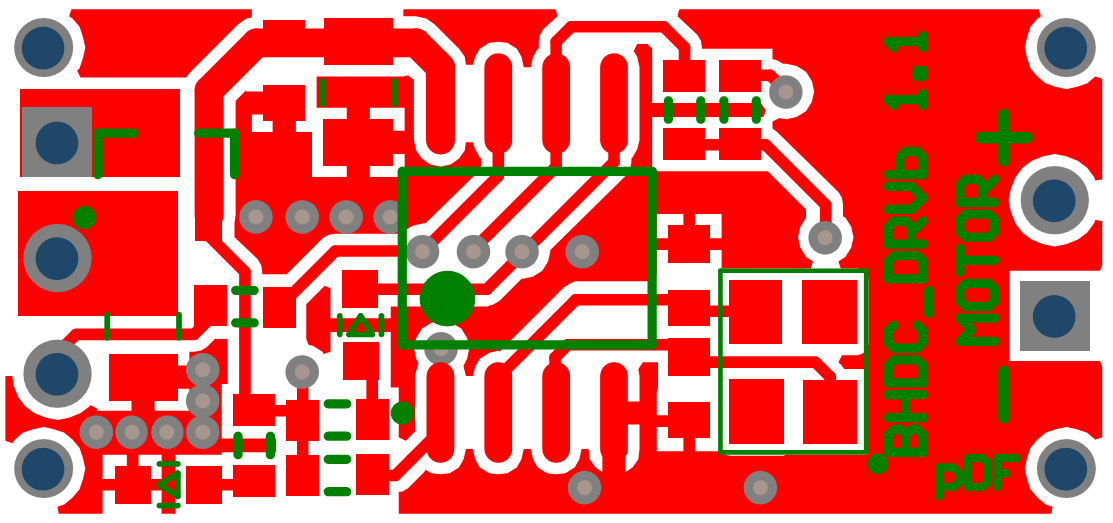
\includegraphics[scale=0.4]{Pictures/MotorDriverPCB_Top.png}
		%\rule{35em}{0.5pt}
		\caption[Sterownik silnika - płytka PCB, warstrwa górna]{Sterownik silnika - płytka PCB, warstwa górna}
	\label{fig:MotorDriverPCB_Top}
\end{figure}


\begin{figure}[H]
	\centering
	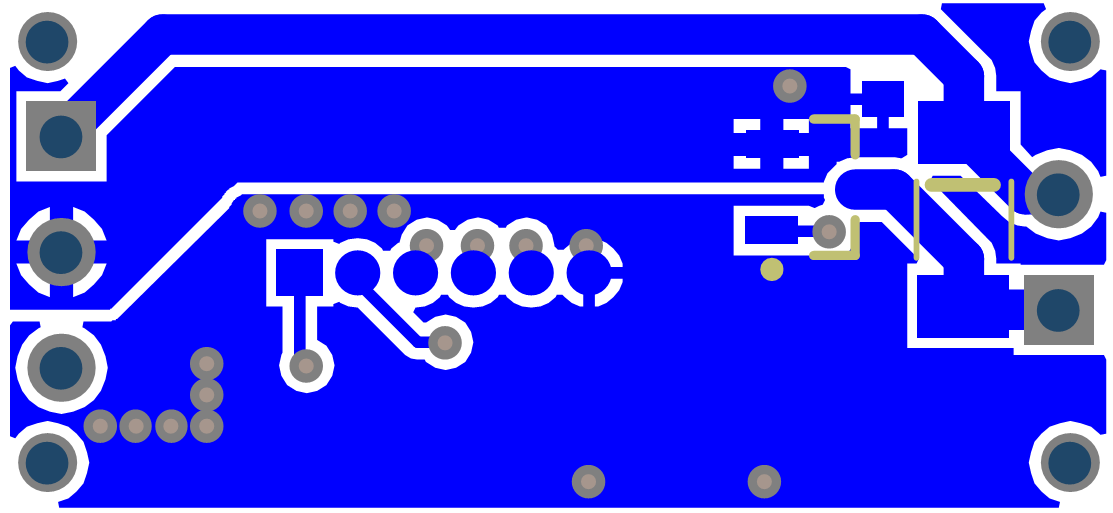
\includegraphics[scale=0.4]{Pictures/MotorDriverPCB_Bottom.png}
		%\rule{35em}{0.5pt}
		\caption[Sterownik silnika - płytka PCB warstwa dolna]{Sterownik silnika - płytka PCB warstwa dolna}
	\label{fig:MotorDriverPCB_Bottom}
\end{figure}

Rysunek ~\ref{fig:MotorDriverPCB_Top} oraz ~\ref{fig:MotorDriverPCB_Bottom} przedstawiają górną i dolną wartstwę płytki PCB sterownika silnika. Na górnej warstwie umieszczono zdecydowaną większość elementów oraz poprowadzono prawie wszystkie sygnały. Na warstwie dolnej umieszczono tranzystor sterujący silnikiem oraz diodę Schottky'ego niwelującą zakłócenia. Przy projektowaniu tej płytki najważniejszą kwestią było prawidłowe poprowadzenie linii zasilania silnika oraz pola masy. Dlatego też na warstwie dolnej widać szeroką ścieżkę doprowadzającą zasilanie z akumulatora do złącza silnika oraz poligon masy analogowej, którym prąd płynący przez silnik będzie wracał do źródła zasilania. Kluczowym aspektem przy prowadzeniu tego poligonu było zadbanie, aby nie przechodził on pod liniami sygnału zegarowego idącymi na wartwie górnej. Dlatego też na warstwie dolnej widać duże pole masy cyfrowej znajdującej się pod większością linii sygnałowych warstwy górnej. Koncentracja elementów na płytce jest stosunkowo duża i wynika z chęci zaprojektowania sterownika o minimalnych rozmiarach. 

\section{Konstrukcja mechaniczna}

Ponieważ autor pracy nie ma doświadczenia w projektowaniu konstrukcji mechanicznych, zdecydowano się na użycie gotowej ramy do kwadrokoptera, opisanej w Internecie. W większości sklepów jedyne ramy dostępne do kupienia przewidziane są do współpracy z silnikami bezszczotkowymi dużej mocy, co kłóci się z wymaganiem technicznym mówiącym o małej mocy silników. W tej sytuacji najprostszym rozwiązaniem było kupienie gotowego kwadrokoptera i wykorzystanie jedynie mechaniki, do której zaprojektowano kontroler lotu i sterowniki silników. 

\begin{figure}[H]
	\centering
	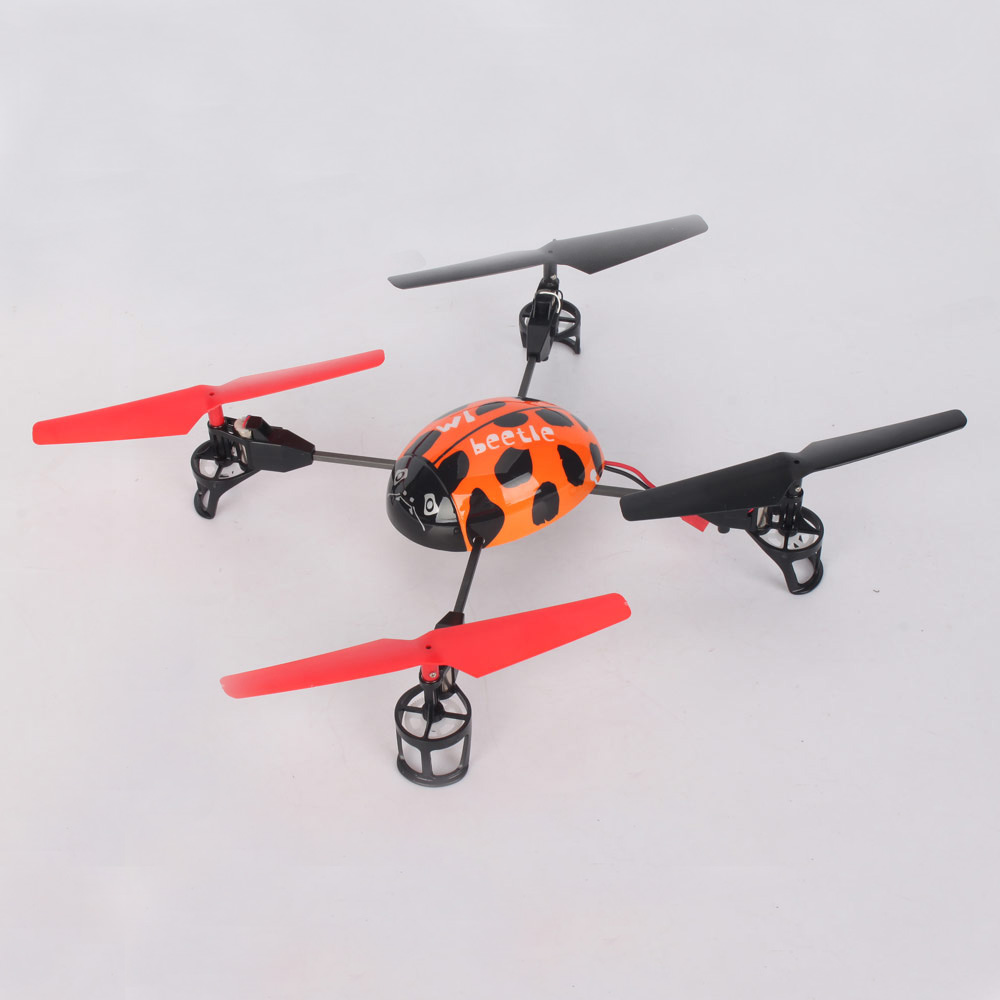
\includegraphics[scale=0.3]{Pictures/Quadro_beetle2.jpg}
		%\rule{35em}{0.5pt}
		\caption[Model kwadrokoptera WL Toys V929]{Model kwadrokoptera WL Toys V929}
	\label{fig:Quadro_beetle2}
\end{figure}

\begin{figure}[H]
	\centering
	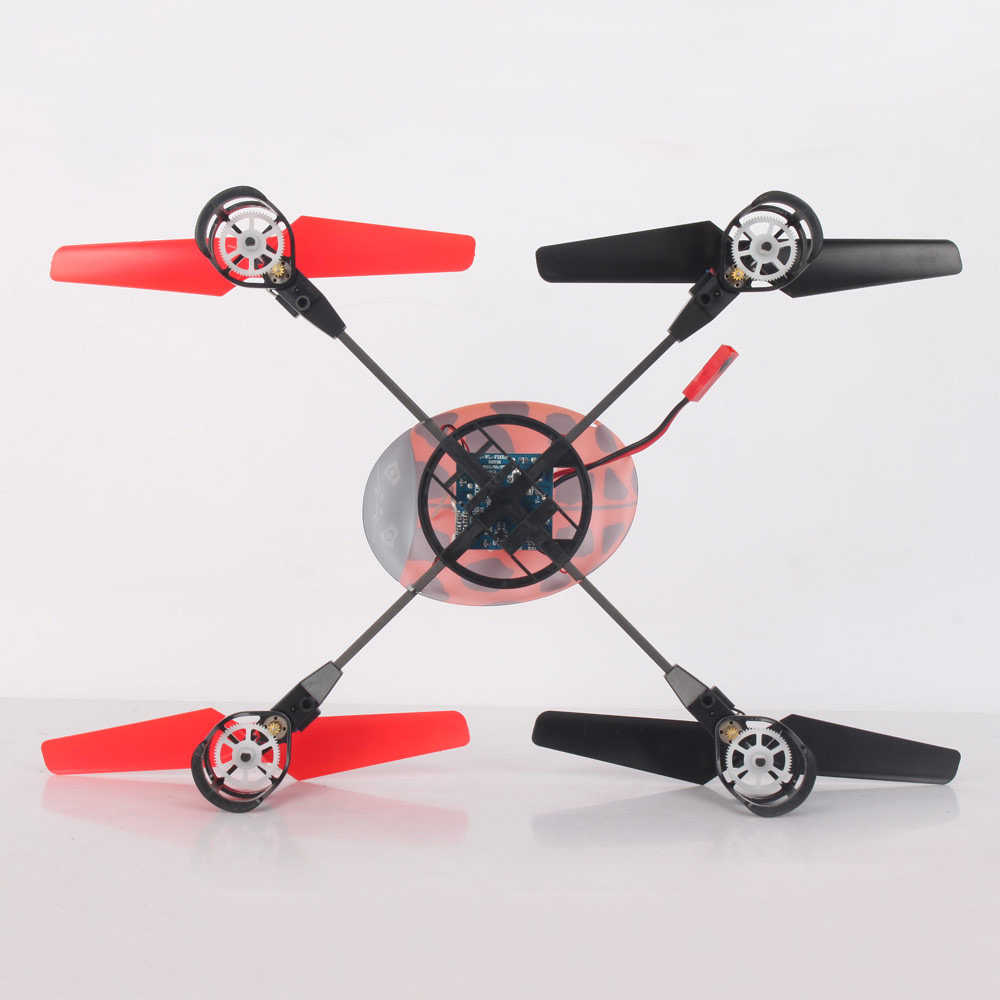
\includegraphics[scale=0.3]{Pictures/Quadro_beetle3.jpg}
		%\rule{35em}{0.5pt}
		\caption[Model kwadrokoptera WL Toys V929 - widok od spodu]{Model kwadrokoptera WL Toys V929 - widok od spodu}
	\label{fig:Quadro_beetle3}
\end{figure}

Po zapoznaniu się z ofertą kwadrokopterów dostepnych w Internecie wybór padł na model WL Toys V929 przedstawiony na rysunku ~\ref{fig:Quadro_beetle2} oraz ~\ref{fig:Quadro_beetle3}. Główne zaletymodelu WL Toys V929 to:

\begin{itemize}
	\item Niska cena przy stosunkowo dużych rozmiarach.
	\item Bardzo duża popularność modelu w sklepach internetowych.
	\item Prosta i wytrzymała konstrukcja mechaniczna ze wspornikami silników wykonanymi z włókien węglowych.
	\item Duża dostępność części zamiennych.
\end{itemize}



Rysunek ~\ref{fig:Quadro_beetle3} przedstawia model od spodu. Widać na nim prostotę konstrukji nośnej kwadrokoptera - cała rama wykonana jest w postaci centralnie umieszczonego pierścienia, do którego przymocowane są cztery wsporniki śmigieł. Na końcach wsporników znajdują się koszyki zawierające silniki wraz z zębatkami oraz śmigłami. Taka konstrukcja mechaniczna pozwala na proste dodawanie własnoręcznie wykonanych pozdespołów elektronicznych (na przykład sterowników silników) i tworzenie gotowej platformy zdolnej do lotu. 

